\section{Overview}
\label{sec:meshing}

\begin{figure}[!t]
\centering
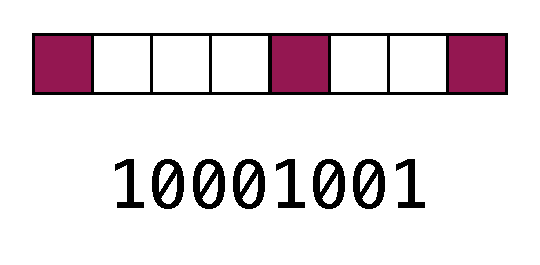
\includegraphics[width=.3\textwidth]{figures/bitmap_bitstring}
\caption{The bitmaps managing the allocated space in a span
  (visualized as allocated objects in the span, top) can be
  represented as bitstrings of 0s and 1s (bottom), where a 1
  corresponds to an allocated object and 0 to free space.}
\label{fig:bitmap-bitstring}
\end{figure}

Meshing is the problem and process of minimizing physical memory use
(measured as resident-set size, or RSS) without modifying allocated
virtual addresses.

A \textit{span} is a contiguous region of memory, and the size of a
span is a multiple of the page size between 4 KiB and 128 KiB.  Each
span allocates objects of a single-size only, for example a 4 KiB span
might hold 32 objects of size 128 bytes.  We can represent a span by a
\textit{bitstring}, a string with a 1 for an allocated object at that
offset from the start of the span and 0 otherwise.  The length of the
bitstring is the number of objects that span holds.

We say $t$ spans \textit{mesh} iff the logical-AND of their bitstrings
($s_i$) of length $t$ is zero. INCORRECT? THIS LETS US MESH TWO 11111 STRINGS WITH ONE 00000 STRING FOR INSTANCE. Formally:

\begin{align}
  \forall k \in [0, b-1]. \sum_{0 \leq i \leq t} s_i[k] \leq 1
\end{align}

This definition characterizes the constraints of the technique by which 
meshing is possible, wherein two or more spans are meshed or "stacked" 
on top of each other.  Each object in the resulting meshed span resides at the same 
offset as it did in its original span, as in Figure 2.  This is only possible when no two spans
have objects at the same offset.  After this process all objects reside
in a single span, and all other spans are empty and can be used anew
for allocation.

The layout and management of a program's heap guide how we consider
meshing.  In a running program, the heap is managed as a number of
different \textit{size classes} along with a region consisting of
large allocations.  Allocations are fulfilled from the smallest size
class they fit in (e.g. an allocation request for 50 bytes is
satisfied by the 64-byte size class), and objects larger than 16 KiB
are individually served from the large allocation region.

We treat each size class as an independent instance of the meshing
problem, and large allocations are not meshed.  As large allocations
are all many multiples of the page size significant fragmentation
between them does not exist.  The number of size-classes is fixed at
compilation time and constant during the execution of a program.

From here, we consider meshing as dealing with a single size-class,
and refer to all spans within this size class as $S$.  If we want to
mesh the entire heap, this means solving $n$ instances of the meshing
problem, where $n$ is the number of size classes.


\begin{figure}[!t]
  \centering
  \begin{subfigure}[t]{.5\textwidth}
    \centering
    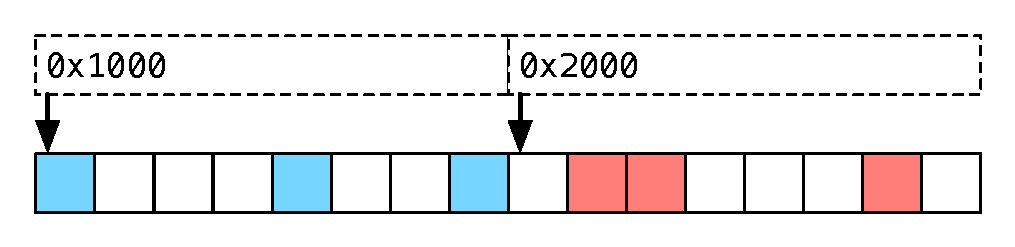
\includegraphics[width=\textwidth]{figures/before_meshing}
    \caption{Two adjacent spans that are candidates for meshing.}
  \end{subfigure}%
  ~

  \begin{subfigure}[t]{.5\textwidth}
    \centering
    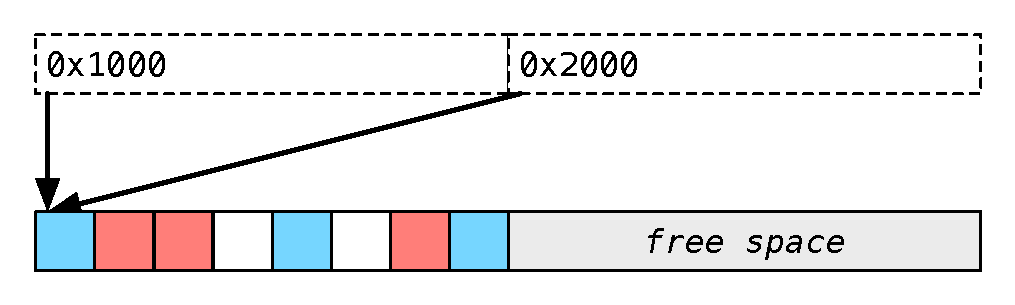
\includegraphics[width=\textwidth]{figures/after_meshing}
    \caption{After meshing, both virtual spans refer to the same
      physical \newline span, with live objects interleaved.}
  \end{subfigure}
  \caption{Virtual and physical memory layout before and after
    meshing.  After meshing, physical span occupancy has increased
    from 37.5\% to 75\% and one physical span has been returned to the
    OS for reuse.}
  \label{fig:meshing}
\end{figure}

Finally, meshing relies on the fact that there are two types of spans,
virtual and physical.  A \textit{virtual} span refers to the memory
addresses visible to the program being executed, while a
\textit{physical} span corresponds to the area in memory where
allocated objects live.  Meshing is concerned with minimizing the
count of in-use physical spans without modifying or moving virtual
spans.  As noted in Section~\ref{sec:introduction}, we cannot change
or modify virtual addresses returned from the allocator, as we do
not have a way to enumerate and update all references the program has
stored.  Since the last two digits of a virtual address directly specify the offset of the referenced object in the span, objects cannot
be safely relocated to a different offset, leading to our 

Allocated objects and free space within a span are tracked by the
memory allocator as a bitmap (see Section~\ref{sec:allocator}) -- the
in-memory representation of a bitstring.  For example, for objects of
size 32 and a span size of 4 KiB, the span can hold 128 32-byte
objects, so allocated objects are be tracked with a 128-bit bitmap.
Each allocated object in a running program has a unique
\textit{(bitmap, offset)} tuple.  Bitmaps are between 8 and 256-bits
in length.

We can therefore think of the meshing problem as that of partitioning
a set of equal-length bitstrings such that the bitstrings in each subset
mesh.  An optimal partition would minimize the number of such subsets.
This abstraction allows us to analyze the complexity of this computational
task in Section~\ref{sec:theory}.